<<<<<<< HEAD

\newcommand{\I}{\mathcal{I}}
\newcommand{\M}{\mathcal{M}}
\newcommand{\timestr}{\mathcal{T}}

\newcommand{\D}{\mathcal{D}}
\newcommand{\C}{\mathcal{C}}

%old, compatibility reasons
\newcommand{\U}{\mathbf{U}}
\newcommand{\Snc}{\mathbf{S}}
\newcommand{\T}{\mathbf{T}}
\newcommand{\R}{\mathbf{R}}

\newcommand{\Nat}{\mathbb{N}}
\newcommand{\Z}{\mathbb{Z}}
\newcommand{\Real}{\mathbb{R}}
\newcommand{\Q}{\mathbb{Q}}

%old, compatibility reasons

\newcommand{\X}[1]{\mathbf{X}\left(#1\right)}
\newcommand{\Y}[1]{\mathbf{Y}\left(#1\right)}

%\newcommand{\X}{\mathbf{X}}
%\newcommand{\Y}{\mathbf{Y}}


\newcommand{\Zed}{\mathbf{Z}}
\newcommand{\Lng}{\mathscr {L}}
\newcommand{\iFF}{\Leftrightarrow}
\newcommand{\niFF}{\nLeftrightarrow}
\newcommand{\SNC}{{\mathcal S}}
\newcommand{\TRG}{{\mathcal T}}
\newcommand{\zot}{$\mathds{Z}$ot}
%old, compatibility reasons
\newcommand{\G}[1]{\mathbf{G}\left(#1\right)}
\newcommand{\F}[1]{\mathbf{F}\left(#1\right)}
%\newcommand{\Q}{\mathbb{Q}}

\newcommand{\triple}[3]{(#1, #2, #3)}
\newcommand{\pair}[2]{(#1, #2)}
\newcommand{\siff}{\Leftrightarrow}
\newcommand{\A}{\mathcal{A}}
\newcommand{\aX}{\mathrm{X}}
\newcommand{\aY}{\mathrm{Y}}
\newcommand{\x}{\mathbf{x}}
\newcommand{\eqdef}{\stackrel{\mbox{\begin{tiny}def\end{tiny}}}{=}} % =def=
\newcommand{\iFFdef}{\stackrel{\mbox{\begin{tiny}def\end{tiny}}}{\iFF}}
% =def=
\newcommand{\step}[1]{\xrightarrow{#1}}

\newcommand{\pspace}{\textsc{PSpace}}


\makeatletter
\def\Eqlfill@{\arrowfill@\Relbar\Relbar\Relbar}
\newcommand{\longmodels}[1][]{\,|\!\!\!\ext@arrow 0359\Eqlfill@{#1}}
\makeatother

\newcommand{\symodels}{\longmodels{\mbox{\it{\tiny sym}}}}

\newcommand{\intervaLii}[2]{[#1,#2]}
\newcommand{\intervaLie}[2]{[#1,#2)}
\newcommand{\intervaLee}[2]{(#1,#2)}

\newcommand{\interval}[2]{\langle #1,#2 \rangle}

\newcommand{\set}[1]{\{ #1 \}}

\newcommand{\tsys}[1]{\mathcal{S}(#1)}


\newcommand{\lapp}[1]{\lfloor #1 \rfloor}
\newcommand{\happ}[1]{\lceil #1 \rceil}


\newcommand{\first}[2]{(H_{#1}\vee L_{#1}) \wedge(\neg(H_{#1}\vee L_{#1}) \Snc (#2))}



\newcommand{\pname}[1]{\ensuremath{\textit{#1}}}
\newcommand{\on}{\pname{on}}
\newcommand{\off}{\pname{off}}
\newcommand{\lon}{\pname{l}}
\newcommand{\test}{\pname{test}}
\newcommand{\resetc}{\pname{reset-c}}
\newcommand{\turnoff}{\pname{turnoff}}




\newcommand{\edge}[1]{\texttt{#1}}
\newcommand{\enabled}[1]{\texttt{e}_{#1}}

\newcommand{\visit}[1]{\mathit{visit}(#1)}
\newcommand{\inv}[1]{\mathit{inv}(q_{#1})}


\newcommand{\intg}[1]{\lfloor#1\rfloor}
\newcommand{\fract}[1]{\mathit{frac(#1)}}



%%%%%%%%%%%%%%% STORM MODEL COMMANDS


\newcommand{\ori}{\mathtt{orig}}
%commands with single parameter
\newcommand{\p}[1]{\mathtt{process}_{#1}}
\newcommand{\ta}[1]{\mathtt{take}_{#1}}
\newcommand{\e}[1]{\mathtt{emit}_{#1}}
\newcommand{\add}[1]{\mathtt{add}_{#1}}
\newcommand{\f}[1]{\mathtt{fail}_{#1}}
\newcommand{\buf}[1]{\mathtt{buffer}_{#1}}
\newcommand{\startf}[1]{\mathtt{startFailure}_{#1}}
\newcommand{\startid}[1]{\mathtt{startIdle}_{#1}}
\newcommand{\id}[1]{\mathtt{idle}_{#1}}
\newcommand{\cl}[1]{\mathtt{clock}_{#1}}
\newcommand{\cltf}[1]{ \cl{to\f{#1}}}
\newcommand{\ph}[1]{\mathtt{phase}_{#1}}

%commands with two parameters (index, rate)
\newcommand{\pr}[2]{\p{#1}(#2)}
\newcommand{\tar}[2]{\ta{#1}(#2)}
\newcommand{\er}[2]{\e{#1}(#2)}
\newcommand{\addr}[2]{\add{#1}(#2)}
\newcommand{\ra}[1]{r_{\add{#1}}}
\newcommand{\rp}[1]{r_{\p{#1}}}
\newcommand{\re}[1]{r_{\e{#1}}}
\newcommand{\rt}[1]{r_{\ta{#1}}}
\newcommand{\rf}[1]{r_{\mathtt{failure}_{#1}}}
\newcommand{\rff}[2]{r_{\mathtt{failure}_{#1#2}}}
\newcommand{\rr}[1]{r_{\mathtt{replay}_{#1}}}
\newcommand{\reb}[1]{\bar{r}_{\e{#1}}}
\newcommand{\rth}[1]{\hat{r}_{\ta{#1}}}
\newcommand{\reh}[1]{\hat{r}_{\e{#1}}}

\newcommand{\tph}[2]{t_{\ph{#1}}^{#2} }

	

%\textbf{@Marcello,Francesco: we should also probably elaborate on the kind of verification technique we are using and how that can help in evaluating the topology.. remember here we do not have the DICE restriction so we can mention any kind of analysis that it would be possible to run, also analyses that are currently in the hands of other DICE partners!!}

%\begin{itemize}
%\item we can use the ATC case study as much as we want - that yields already three topologies that we can infer
%\item ATC has agreed that we can mention their role in this exercise, I also showed them the topology that we elicited basically with OSTIA and they already made considerations on how to improve it
%\item in the evaluation we should also comment on how OSTIA can help you in visualizing the application topology that you may be considering to use by reusing a big-data application for something else... visualising the application topology and analysing it may allow you to improve it while you are using it as a starting point for your application
%\item another application that we can use is the one that NETF is considering for their own scenario, KILLRWEATHER - \url{https://github.com/killrweather/killrweather}
%\item any additional case that we can run?
%\item what do the results show? do we have a way to quickly quantify the time that is saved by using this approach? e.g., the time that is saved in setting up and running the infrastructure and how much would that time saved have costed these could be valuable evaluation insights
%\end{itemize}
This section elaborates on our evaluation campaign. As previously stated, we evaluated OSTIA through qualitative evaluation and case-study research featuring an open-/closed-source industrial case-study (see Section \ref{cs}) and two open-source case-studies (see Section \ref{os}) on which we also applied complex formal verification (see Section \ref{ver}).

\subsection{Industrial Case-Study}\label{cs}

As previously introduced in Section \ref{ra}, we operated an evaluation of OSTIA running the application on a closed-source cascade of several topologies part of the SocialSensor App. Our industrial partner is having performance and availability outages connected to currently unknown circumstances. Therefore, the objective of our evaluation for OSTIA was twofold: (a) allow our industrial partner to enact continuous architecting of their application with the goal of discovering any patterns or hotspots that may be requiring further architectural reasoning; (b) understand wether OSTIA provided valuable feedback to endure the continuous architecting exercise.

OSTIA output for the SocialSensor topologies is outlined in Fig. \ref{topo1}.

\begin{figure}[H]
		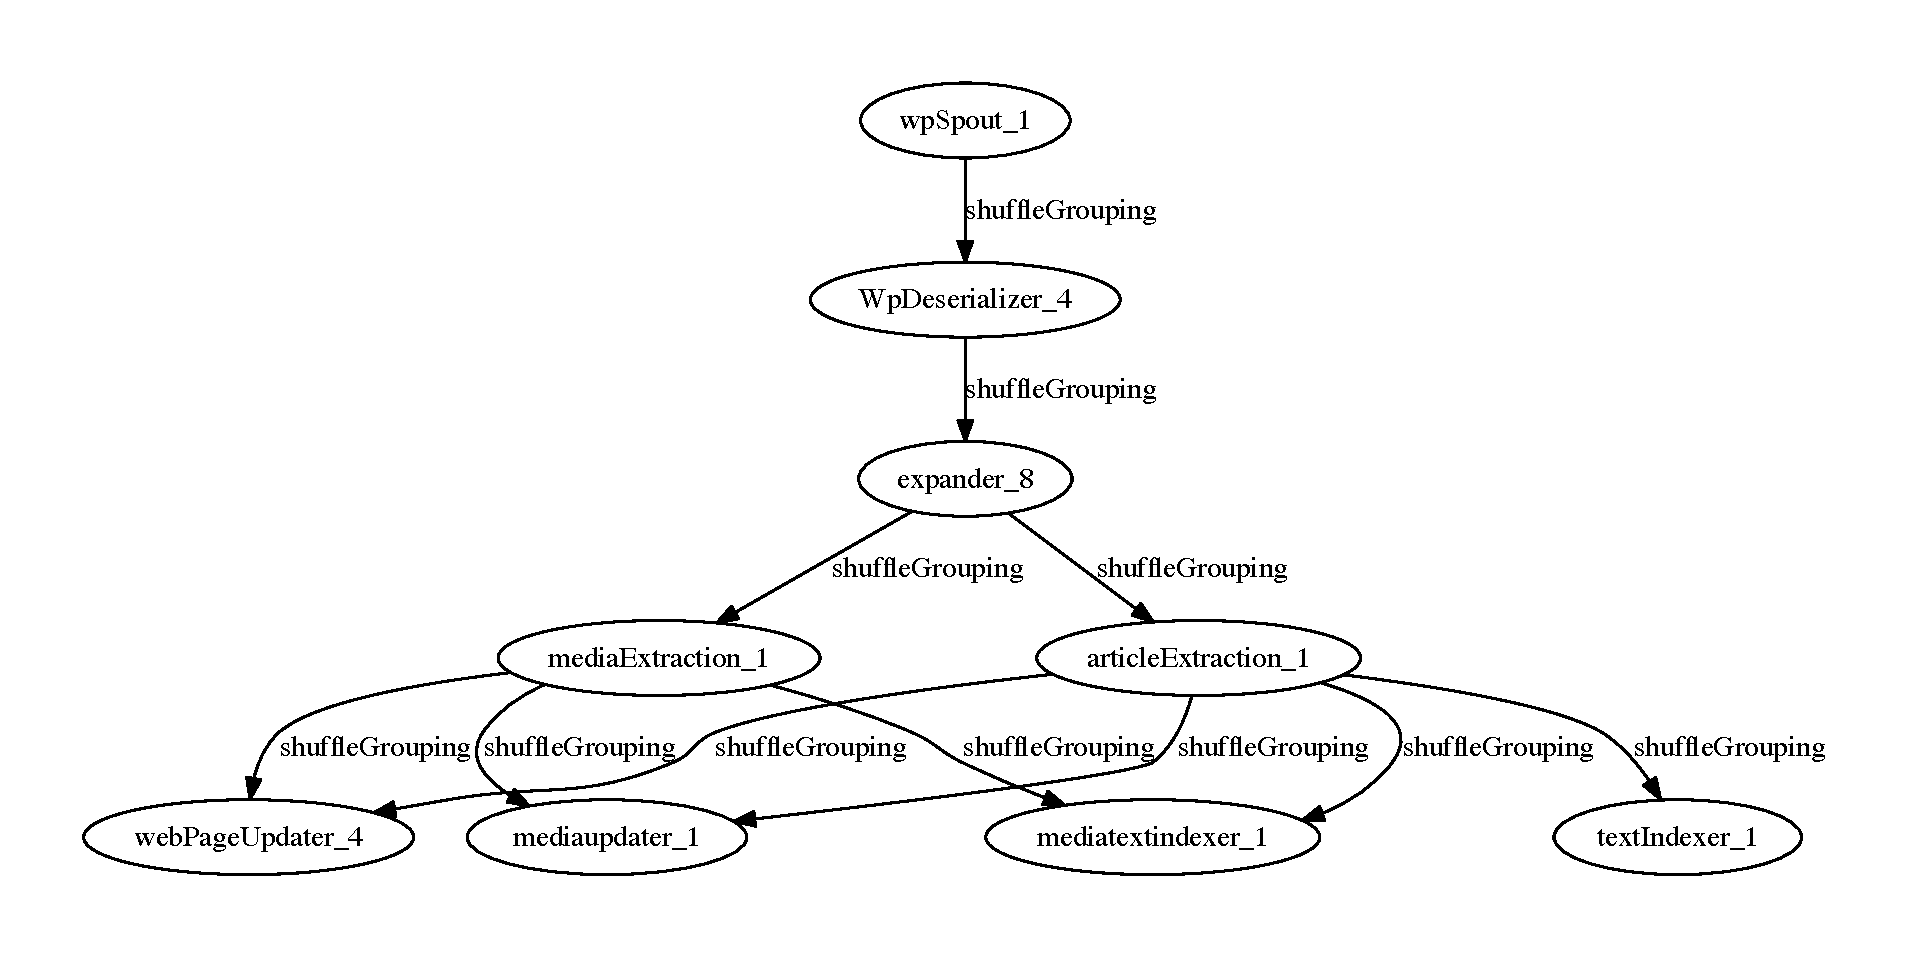
\includegraphics[width=9cm]{images/output/focused_crawler}
		\caption{SocialSensor App, OSTIA sample output.}
		\label{topo1}
\end{figure}

OSTIA findings are as follows:
\begin{itemize}
\item A double instance of the ``Multi-Anchoring" pattern is found around bolt ``expander";
\item An instance of the ``Persistent Data" pattern is found around bolt ``expander" as well;
\item An instance of the ``Computational Funnel" pattern is found around bolt ``expander";
\end{itemize}

as a consequence of these outputs our industrial partner observed that the ``expander" bolt clearly needed additional architectural reasoning. Also, the partner welcomed the idea of using OSTIA as a mechanism to enact continuous architecting of the topology in question as part of the needed architectural reasoning.

Besides this pattern-based evaluation and assessment, OSTIA algorithmic analyses assisted our client in understanding that the topological structure and cascade of the SocialSensor app would be better fit for batch processing rather than streaming, since the partner observed autonomously that too many Database-output spouts and bolts were used in their versions of the SocialSensor topologies. In so doing, the partner is now using OSTIA to drive the refactoring exercise towards a Hadoop Map Reduce\footnote{\url{http://hadoop.apache.org/}} framework for batch processing.

\subsection{Confirming OSTIA Usefulness with Open-Source Case-Studies}\label{os}

\subsection{OSTIA-Based Formal Verification}\label{ver}

\newcommand{\I}{\mathcal{I}}
\newcommand{\M}{\mathcal{M}}
\newcommand{\timestr}{\mathcal{T}}

\newcommand{\D}{\mathcal{D}}
\newcommand{\C}{\mathcal{C}}

%old, compatibility reasons
\newcommand{\U}{\mathbf{U}}
\newcommand{\Snc}{\mathbf{S}}
\newcommand{\T}{\mathbf{T}}
\newcommand{\R}{\mathbf{R}}

\newcommand{\Nat}{\mathbb{N}}
\newcommand{\Z}{\mathbb{Z}}
\newcommand{\Real}{\mathbb{R}}
\newcommand{\Q}{\mathbb{Q}}

%old, compatibility reasons

\newcommand{\X}[1]{\mathbf{X}\left(#1\right)}
\newcommand{\Y}[1]{\mathbf{Y}\left(#1\right)}

%\newcommand{\X}{\mathbf{X}}
%\newcommand{\Y}{\mathbf{Y}}


\newcommand{\Zed}{\mathbf{Z}}
\newcommand{\Lng}{\mathscr {L}}
\newcommand{\iFF}{\Leftrightarrow}
\newcommand{\niFF}{\nLeftrightarrow}
\newcommand{\SNC}{{\mathcal S}}
\newcommand{\TRG}{{\mathcal T}}
\newcommand{\zot}{$\mathds{Z}$ot}
%old, compatibility reasons
\newcommand{\G}[1]{\mathbf{G}\left(#1\right)}
\newcommand{\F}[1]{\mathbf{F}\left(#1\right)}
%\newcommand{\Q}{\mathbb{Q}}

\newcommand{\triple}[3]{(#1, #2, #3)}
\newcommand{\pair}[2]{(#1, #2)}
\newcommand{\siff}{\Leftrightarrow}
\newcommand{\A}{\mathcal{A}}
\newcommand{\aX}{\mathrm{X}}
\newcommand{\aY}{\mathrm{Y}}
\newcommand{\x}{\mathbf{x}}
\newcommand{\eqdef}{\stackrel{\mbox{\begin{tiny}def\end{tiny}}}{=}} % =def=
\newcommand{\iFFdef}{\stackrel{\mbox{\begin{tiny}def\end{tiny}}}{\iFF}}
% =def=
\newcommand{\step}[1]{\xrightarrow{#1}}

\newcommand{\pspace}{\textsc{PSpace}}


\makeatletter
\def\Eqlfill@{\arrowfill@\Relbar\Relbar\Relbar}
\newcommand{\longmodels}[1][]{\,|\!\!\!\ext@arrow 0359\Eqlfill@{#1}}
\makeatother

\newcommand{\symodels}{\longmodels{\mbox{\it{\tiny sym}}}}

\newcommand{\intervaLii}[2]{[#1,#2]}
\newcommand{\intervaLie}[2]{[#1,#2)}
\newcommand{\intervaLee}[2]{(#1,#2)}

\newcommand{\interval}[2]{\langle #1,#2 \rangle}

\newcommand{\set}[1]{\{ #1 \}}

\newcommand{\tsys}[1]{\mathcal{S}(#1)}


\newcommand{\lapp}[1]{\lfloor #1 \rfloor}
\newcommand{\happ}[1]{\lceil #1 \rceil}


\newcommand{\first}[2]{(H_{#1}\vee L_{#1}) \wedge(\neg(H_{#1}\vee L_{#1}) \Snc (#2))}



\newcommand{\pname}[1]{\ensuremath{\textit{#1}}}
\newcommand{\on}{\pname{on}}
\newcommand{\off}{\pname{off}}
\newcommand{\lon}{\pname{l}}
\newcommand{\test}{\pname{test}}
\newcommand{\resetc}{\pname{reset-c}}
\newcommand{\turnoff}{\pname{turnoff}}




\newcommand{\edge}[1]{\texttt{#1}}
\newcommand{\enabled}[1]{\texttt{e}_{#1}}

\newcommand{\visit}[1]{\mathit{visit}(#1)}
\newcommand{\inv}[1]{\mathit{inv}(q_{#1})}


\newcommand{\intg}[1]{\lfloor#1\rfloor}
\newcommand{\fract}[1]{\mathit{frac(#1)}}



%%%%%%%%%%%%%%% STORM MODEL COMMANDS


\newcommand{\ori}{\mathtt{orig}}
%commands with single parameter
\newcommand{\p}[1]{\mathtt{process}_{#1}}
\newcommand{\ta}[1]{\mathtt{take}_{#1}}
\newcommand{\e}[1]{\mathtt{emit}_{#1}}
\newcommand{\add}[1]{\mathtt{add}_{#1}}
\newcommand{\f}[1]{\mathtt{fail}_{#1}}
\newcommand{\buf}[1]{\mathtt{buffer}_{#1}}
\newcommand{\startf}[1]{\mathtt{startFailure}_{#1}}
\newcommand{\startid}[1]{\mathtt{startIdle}_{#1}}
\newcommand{\id}[1]{\mathtt{idle}_{#1}}
\newcommand{\cl}[1]{\mathtt{clock}_{#1}}
\newcommand{\cltf}[1]{ \cl{to\f{#1}}}
\newcommand{\ph}[1]{\mathtt{phase}_{#1}}

%commands with two parameters (index, rate)
\newcommand{\pr}[2]{\p{#1}(#2)}
\newcommand{\tar}[2]{\ta{#1}(#2)}
\newcommand{\er}[2]{\e{#1}(#2)}
\newcommand{\addr}[2]{\add{#1}(#2)}
\newcommand{\ra}[1]{r_{\add{#1}}}
\newcommand{\rp}[1]{r_{\p{#1}}}
\newcommand{\re}[1]{r_{\e{#1}}}
\newcommand{\rt}[1]{r_{\ta{#1}}}
\newcommand{\rf}[1]{r_{\mathtt{failure}_{#1}}}
\newcommand{\rff}[2]{r_{\mathtt{failure}_{#1#2}}}
\newcommand{\rr}[1]{r_{\mathtt{replay}_{#1}}}
\newcommand{\reb}[1]{\bar{r}_{\e{#1}}}
\newcommand{\rth}[1]{\hat{r}_{\ta{#1}}}
\newcommand{\reh}[1]{\hat{r}_{\e{#1}}}

\newcommand{\tph}[2]{t_{\ph{#1}}^{#2} }

	

This section describes the formal modelling and verification employed in OSTIA  which both rely on \textit{satisfiability checking}~\cite{MPS13}, an alternative approach to model-checking.
Instead of an operational model (like automata or transition systems), as in model-checking, 
the system (i.e., a topology in this context) is specified by a formula defining their executions over time and properties are verified by proving that the system logically entails them.

The logic we use is Constraint LTL over clocks (CLTLoc)~\cite{BRS15} which is a semantic restriction of Constraint LTL (CLTL)~\cite{DD07} allowing atomic formulae over $(\mathbb{R}, \set{<,=})$ where the arithmetical variables behave like clocks of Timed Automata (TA)~\cite{timed}.
A clock $x$ measures the time elapsed since the last time when $x=0$ held, i.e., since the last ``reset'' of $x$.
Clocks are interpreted over Reals and their value can be tested with respect to a positive integer value.
%
Let $X$ be a finite set of clock variables $x$ over $\Real$ and $AP$ be a finite set of atomic propositions $p$.
CLTLoc formulae are defined as follows:
\begin{equation*}%\small
  \phi :=
  \begin{gathered}
    p \mid x\sim c \mid \phi \wedge \phi \mid \neg \phi \mid
   \X{\phi} \mid \Y{\phi} %\mid \Zed\phi
\mid \phi\U\phi \mid \phi\Snc\phi
  \end{gathered}
\end{equation*}
where %$p\in AP$, $x \in V$, 
$c \in \Nat$ and $\sim \in \set{<,=}$, $\bullet$, $\circ$, $\U$ and $\Snc$ are the usual ``next'', ``previous'', ``until'' and ``since''.
%The semantics of CLTLoc is defined with respect to $(\Real, \set{<,=})$ and $\pair{\Nat}{<}$, the latter representing positions in time.
A \textit{model} is a pair $\pair{\pi}{\sigma}$, where $\sigma$ is a mapping associating every variable $x$ and position in $\Nat$ with value $\sigma(i,x)$ and $\pi$ is a mapping associating each position in $\Nat$ with subset of $AP$. 
The semantics of CLTLoc is defined as for LTL except for formulae $x\sim c$. 
At position $i\in\Nat$, $ \pair{\pi}{\sigma}, i \models x\sim c \textbf{ iff }  \sigma(i, x)\sim c$.
A formula is \textit{satisfiable} if it has a model.

The standard technique to prove the satisfiability of CLTL and CLTLoc formulae is based on of B\"uchi automata \cite{DD07,BRS15} %the evidence has turned out that it may be rather expensive in practice, even in the case of LTL (the size of the automaton is exponential with respect to the size of the formula).
but, for practical implementation, Bounded Satisfiability Checking (BSC)~\cite{MPS13} avoids the onerous construction of automata.
By unrolling the semantics of a formula for a finite number $k>0$ of steps, 
the outcome of a BSC problem is either an infinite ultimately periodic model or unsat.
\cite{BRS15} shows that BSC for CLTLoc is complete and that is reducible to a decidable Satisfiability Modulo Theory (SMT) problem. 
A CLTLoc formula can be translated into the decidable theory of quantifier-free formulae with equality and uninterpreted functions combined with the theory of Reals over $(\Real,<)$. %, written QF-EUF$(\Real,<)$.

CLTLoc allows the specification of temporal constraints using clock variables ranging over $\Real$, whose value is not abstracted.
Clock variables represent, in the logical language and with the same precision, physical (dense) clocks.
They appear in formulae of the form $x \sim c$ to express a bound $c$ on the delay measured by clock $x$. 
Clocks are associated with specific events to measure time elapsing over the execution.
As they are reset when the associated event occurs, in any moment, the clock value represents the time elapsed since the previous reset and corresponds to the elapsed time since the last occurrence of the event associated to it.
We use such constraints to define, for instance, the time delay required to process tuples or between two node failures.

%Modeling topologies requires to express by formulae emitting rates which measure the number of tuples emitted by a spout node per time unit.
%***TBC

%Verification techinques:
%\begin{itemize}
%\item Safety Verification
%\item Performance analysis	
%\end{itemize}
%A \textit{safety} property is intuitively defined in the formal verification context as a property stating that something ``bad'' will \textit{never} happen during execution.\cite{lamport1}
%Cassical examples of safety properties are deadlock freedom and mutual exclusion, where the ``bad'' behaviour is respectively the deadlock occurrence and the simultaneous execution of a critical section.
%One of the most important requirements for streaming systems is guaranteeing low latency while maintaining high throughput. 
%In a distributed  --> Motivare questione delle code!
%

%
%\subsection{Storm Formal Model}
%\label{sec:storm-model}
%To perform our verification tasks we defined a formal model expressed in CLTLoc with discrete variables. The resulting model is a non-deterministic infinite state system.

% MOVED BEFORE
%%%\subsubsection{OSTIA Models: a Formal Interpretation}
%%%We started by understanding and capturing the behaviors of both spouts and bolts. 
%%%After choosing the level of abstraction of our model we simplified those behaviors accordingly, in order to formalize them as finite state machines. The purpose of this first activity was to define the possible operations and the allowed orderings of such operations.
%%%We then extended the model by taking into account the message buffers (or queues) and the quantity of tuples that are exchanged through the topology.
%%%In addition to the correct ordering of the operations, we decided to introduce more specific temporal constraints into the model, in order to limit the time spent by the system in each state (or processing phase) and to elaborate the concept of \textit{rate}, intended as ``number of times an event is occurring every time unit''.\\

%\subsubsection{Assumptions and  level of abstraction}
%We made several assumptions and abstractions while building the model:

Building on top of the above framework,  a formal interpretation of the Storm (meta-)model requires several abstractions and assumptions.

%For example, some deployment details, such as the number of worker nodes and features of the underlying cluster, are abstracted away. 
%There is a single queuing layer: every bolt has a unique incoming queue and no sending queue, while the worker queues are not represented. In the same way, each bolt/spout has a single output stream.
%Moreover, the content of messages is not relevant: all the tuples have the same fixed size and we represent only quantity of tuples moving through the system.


\begin{itemize}
	\item some deployment details, e.g., the number of worker nodes and features of the underlying cluster, are abstracted away;
	\item each bolt/spout has a single output stream;
	\item %we simplified the message buffer system, assuming that 
	there is a single queuing layer: every bolt has a unique incoming queue and no sending queue, while the worker queues are not represented;
	\item every operation is performed within minimum and maximum thresholds of time;
	\item %we do not take into account 
	the content of the messages is not relevant: all the tuples have the same fixed size and we represent only quantity of tuples moving through the system;
\end{itemize}

%\subsubsection{Model Formalization}
A Storm Topology is a directed graph $\mathbf{G} = \{ \mathbf{N}, Sub\}$ where the set of nodes $\mathbf{N} = \mathbf{S}\bigcup \mathbf{B}$ includes in the sets of spouts (\textbf{S}) and bolts (\textbf{B}) and %the set of edges $\mathbf{E} = \{ Sub_{i,j} | i \in \mathbf{B}, j \in \{\mathbf{S}\bigcup \mathbf{B}\} \}$ 
$Sub\subset\mathbf{N}\times\mathbf{N}$ defines how the nodes are connected each other via the subscription relation. Pair $(i,j)\in Sub$ indicates that ``bolt $i$ subscribes to the streams emitted by the spout/bolt $j$''. 
Spouts cannot subscribe to other nodes in the topology.
Each bolt has a receive queue where the incoming tuples are collected before being read and processed. % by the node.
The queues have infinite size and the level of occupation of each $j^{th}$ queue is described by the variable $q_j$. %\footnote{Spouts have no queues, by definition.}
Spouts have no queues, and 
each spout can either \textit{emit} tuples into the topology or stay \emph{idle}.
Each bolt can be in \emph{idle} state, in \emph{failure} state or in  \emph{processing} state.  While in the processing state, the bolt first reads tuples from its receive queue (\textit{take} action), then it performs its transformation (\textit{execute} action) and finally it \textit{emits} the output tuples in its output streams. \\
\begin{figure}[tb]
\centering
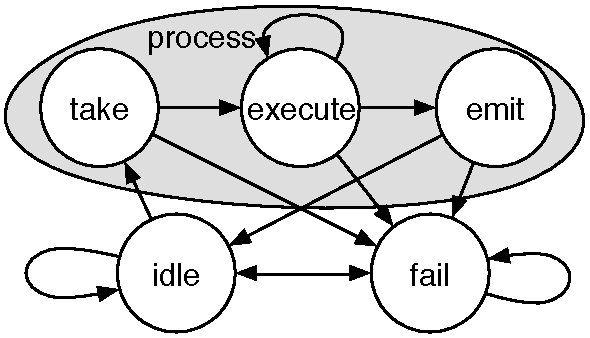
\includegraphics[width=0.7\linewidth]{images/bolt-fsm}
\caption{Finite state automaton describing bolt states.}
\label{figure-fsa}
\end{figure}

%\begin{figure}
%	\centering	
%	\begin{tikzpicture}[->,>=stealth',shorten >=1pt,auto,node distance=2.5cm,semithick, every node/.style={scale=0.55}]
%	
%	\tikzstyle{every state}=[fill=white,text=black,minimum width={width("execute")+10pt}]
%	
%	
%	\node[state]            (I) {$idle$};  
%	\node[state]         (T) [above right of=I] {$take$};  
%	\node[state]         (E) [right of=T] {$execute$};
%	\node[state]         (F) [below right of=I] {$fail$};
%	\node[state]         (EM) [right of=F] {$emit$};
%	
%	\path (I) edge              node {} (T)
%	edge              node {} (F)
%	edge [loop above]  node {} (I)
%	(E) edge [loop right] node {} (E)
%	edge              node {} (EM)
%	(T) edge              node {} (E)
%	edge              node {} (F)
%	(EM) edge             node {} (I)
%	edge              node {} (F)
%	(F) edge [loop below]  node {} (F);
%	edge [bend right]  node {} (I);
%	\end{tikzpicture}
%	\caption{Finite state automaton describing bolt states.}
%	\label{figure-fsa}
%\end{figure}
%To give an idea about how the model is formalized, 
We provide, as an example, one of the formulae defining the processing state. Formula \ref{formula:1} can be read as \textit{``for all bolts: if a bolt j is processing tuples, then it has been processing tuples since it took those tuples from the queue, (or since the origin of the events), and it will keep processing those tuples until it will either emit them or fail. Moreover, the bolt is not in a failure state''.}
\begin{align}
\small
%
\bigwedge_{
	i \in \mathbf{B} } 
\left( 
\begin{array}{l}
\p{i} \Rightarrow \\
\p{i} \, \Snc \, ( \ta{i} \lor (\ori \land \p{i})) \land \\
\p{i} \, \U \, (\e{i} \lor \f{i}) \land \lnot \f{i} 
\end{array}
\right) \label{formula:1} 
%
\end{align}
The number of tuples emitted by a bolt depends on the number of incoming tuples. The ratio $\frac{\#output\_tuples}{\#input\_tuples}$ %is used to 
expresses the ``kind of function''  performed by the bolt and is given as configuration parameter. 
All the emitted tuples are then added to the receive queues of the bolts subscribing to the emitting nodes.
In the same way, whenever a bolt reads tuples from the queue, the number of elements in queue decreases. To this end, formula \ref{formula:2}, imposes that \textit{``if a bolt takes elements from its queue, the number of queued elements in the next time instant will be equal to the current number of elements plus the quantity of tuples being added (emitted) from other connectd nodes minus the quantity of tuples being read''.}
\begin{align}\small
%
\bigwedge_{
	\begin{subarray}{c}
	\,j \in B
	\end{subarray}
} &( \ta{j}{}  \Rightarrow (\aX q_j = q_j + \ra{j} - \rt{j} )) \label{formula:2}
%
\end{align}
These functional constraints are fixed for all the nodes and they are not configurable.
%What is configurable and can be tuned changing the parameters of the model is everything concerning 
The structure of the topology, the parallelism level of each node, the bolt function and the non-functional requirements, as, for example, the time needed for a bolt in order to process a tuple, the minimum and maximum time between failures and the spout emitting rate are configurable parameters of the model.
Currently, the verification tool accepts %as configuration format 
a JSON file containing all the configuration parameters.
OSTIA supports such format and is able to extract from static code analysis a partial set of features, and an almost complete set of parameters after monitoring a short run of the system. The user can complete the JSON file by adding some verification-specific settings.


